
  \subsection{Programação Dinâmica}

    Programação dinâmica é uma estratégia de construção de algoritmos que 
    possui uma grande eficácia na resolução de problemas de otimização combinatória.
    Em outras palavras, essa estratégia é ideal, quando o problema original 
    é divido em subproblemas, que se repetem, logo podem ser memorizados para 
    evitar recálculo.

    Antes de aplicar essa técnica, o problema precisa atender duas propriedades:
    um problema com subproblemas(Overlapping subproblems) e uma subestrutura ideal
    (Optimal substructure).

    \begin{itemize}
      \item \textbf{Overlapping subproblems}: Uma característica também presente em divisão 
      e conquista, essa propriedade é presente em problemas, onde este pode ser 
      divido em subproblemas que são reutilizados várias vezes.
      \item \textbf{Optimal substructure}: Um problema possui uma subestrutura ideal, quando 
      uma solução ótima pode ser construída, usando solução ótima para os seus subproblemas.
    \end{itemize}

    Para melhor exemplificar esses conceitos, vamos analisar um clássico problema da computação, 
    e também um caso perfeito para ilustrar a estratégia de programação dinâmica.

    \newpage

    \subsubsection{Fibonnaci}

    Descobrido pelo matemático italiano do século 12, Leonardo Fibonacci, a sequência 
    fibonnaci é uma sucessão de números que aparece codificada nos mais diversos fenômenos 
    da natureza(spiral de galáxias, ciclone, conchas e vários outros). Na computação, temos 
    o problema de criar um algoritmo capaz de calcular o n° número da sequência fibonnaci.

    \begin{figure}[ht]
      \centering
      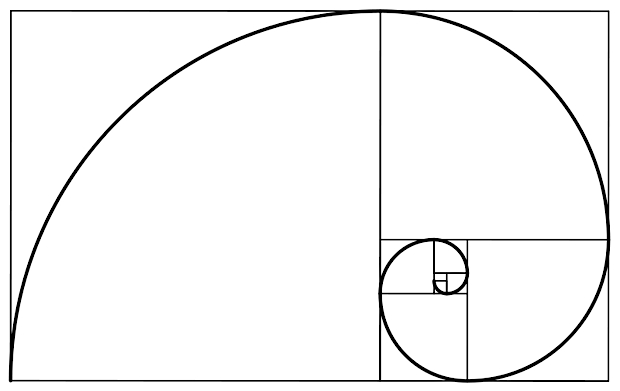
\includegraphics[width=.3\textwidth]{fibonnaci.jpg}
      \caption{Uma imagem ilustrativa da sequência Fibonnaci}
      \label{fig:fibonnaci}
    \end{figure}

    A ideia da resolução desse problema é bem simples, sabendo que a sequência inicia com 0 e 1, os
    próximos números serão sempre a soma dos dois números anteriores. A seguir temos um exemplo 
    de uma implementação ingênua do algoritmo da sequência de fibonnaci. 

    \lstinputlisting[language=Python]{../code/dynamic-programming/fib.py}

    Esta implementação a primeira vista não parece ter nenhum problema. Porém, é quando tentamos 
    executar esse código, que o problema se mostra, o código consegue calcular o 6,7 e 8 número da 
    sequência, porém, o código não consegue calcular o 50° número. 
 
    Para entender a natureza desse problema precisamos entender a complexidade desse código, logo,
    precisamos da árvore de recursão gerada pelo código:

    \newpage 

    \begin{figure}[ht]
      \centering
      \begin{forest}
        for tree={
            grow=south,
            circle, draw, minimum size=3ex, inner sep=2pt,
            s sep=7mm
                }
        [6
            [5
                [4
                  [3
                    [2][1]
                  ]
                  [2]
                ]
                [3
                    [2][1]
                ]
            ]
            [4
                [3
                    [2][1] 
                ]
                [2]
            ]
        ]
        \end{forest}  
        \caption{encontrando o 6° número da sequência fibonnaci}
    \end{figure}

    A primeira coisa a se notar é a complexidade do algoritmo, a 
    árvore formada possui uma altura N(o número que queremos achar da sequência),
    e a cada novo nível da árvore, formamos no máximo, dois novos nós, logo 
    podemos concluir que a complexidade é de $O(2^{n})$, justificando também, porque 
    não conseguimos calcular o 50° número, já que este levaria um tempo 
    equivalente a $2^{50}$.

    Então agora a pergunta fica, como que podemos otimizar essa árvore, de forma 
    que o algoritmo consiga ter um tempo linear, voltando a árvore, podemos observar 
    um padrão recorrente.


    \begin{figure}[ht]
      \centering
      \begin{forest}
        for tree={
            grow=south,
            circle, draw, minimum size=3ex, inner sep=2pt,
            s sep=7mm
                }
        [6
            [5
                [4, tikz={\node[draw,circle,red,fit=()(!1),inner sep=0mm,xshift=3mm]{};} 
                  [3, tikz={\node[draw,circle,red,fit=()(!1),inner sep=0mm,xshift=3mm]{};}
                    [2][1]
                  ]
                  [2]
                ]
                [3 , tikz={\node[draw,circle,blue,fit=()(!1),inner sep=0mm,xshift=3mm]{};} 
                    [2][1]
                ]
            ]
            [4 , tikz={\node[draw,circle,blue,fit=()(!1),inner sep=0mm,xshift=3mm]{};} 
                [3 , tikz={\node[draw,circle,blue,fit=()(!1),inner sep=0mm,xshift=3mm]{};} 
                    [2][1] 
                ]
                [2]
            ]
        ]
        \end{forest}  
        \caption{Vermelho são os passos que são calculados, e o que está em azul é repetido}
    \end{figure}

    Com esse segundo desenho, fica mais evidente que existe passos da recursão que estão repetidos, ou seja,
    o programa acaba resolvendo mais de uma vez os mesmos problemas de forma desnecessária. Em conclusão, para 
    resolver esses problemas, o ideal seria uma estrutura que possa guardar 
    resultados de recursões já feitas, para usar depois, quando o mesmo problema for encontrado, resultando 
    em uma árvore de recursão assim.

    \newpage

    \begin{figure}[ht]
      \centering
      \begin{forest}
        for tree={
            grow=south,
            circle, draw, minimum size=3ex, inner sep=2pt,
            s sep=7mm
                }
        [6
            [5
                [4
                  [3]
                ]
                [3]
            ]
            [4]
        ]
        \end{forest}  
        \caption{Árvore de recursão otimizada}
    \end{figure}

    Com a otimização percebemos que agora a complexidade do 
    código melhorou drasticamente, tendo um resultado de 
    $O(2n)$ visto que é resultado da altura da árvore multiplicado 
    por 2, que pode ser simplificado para apenas $O(n)$.

    Eis então agora o código otimizado:

    \lstinputlisting[language=Python]{../code/dynamic-programming/fib-memoization.py}

    \lstinputlisting[language=Python]{../code/dynamic-programming/fib-tabulation.py}